\section{Event selection}
\subsection{SD and CD}
\begin{enumerate}
	\item Exactly one primary vertex with TPC tracks matched with hits in TOF.
	\item The reconstructed vertex is required to be within $80$~cm of the detector center along the  beam direction.
	\item At least two primary TPC tracks $N^{primary}_{reco}$ matched with hits in TOF and satisfying the selection criteria described in  \ref{chap:trackCut}.
	\item If there are exactly two primary tracks satisfying the above criteria and exactly two global tracks used for vertexing (Table \ref{tab:trackCutVertex}), the longitudinal distance between these tracks $|\Delta z_0|<2$~cm.
\end{enumerate}
\subsection{SD}
\begin{enumerate}
	\item SDT trigger 
	\item RP trigger on only one side of the STAR central detector (veto EAST \&\& WEST)
	\item RP trigger on only UP or DOWN  stations (veto UP \&\& DOWN)
	\item Any signal in small BBC tiles or ZDC on the opposite side of the STAR central detector to the triggered RP station(s).
	\item RP trigger on exactly two RP stations.
	\item Exactly one RP global track in the above RP stations with proton fractional momentum loss $0.02 < \xi < 0.4$.
\end{enumerate}

\subsection{CD}
\begin{enumerate}
	\item CPT2 trigger 
	\item Exactly one RP global track on each side of the STAR central detector with proton fractional momentum loss $0.02 < \xi_1,\xi_2 < 0.4$.
\end{enumerate}
\section{Track selection}\label{chap:trackCut}
For this analysis several track quality cuts are applied as shown in Table \ref{tab:trackCut}. Tracks are required to have at least $25$ fit points, ratio of fit points to possible fit points $N_{fit}/N_{poss}>0.52$, $15$ $dE/dx$ points, transverse impact parameter $d_0<1.5$~cm, and have a $\textrm{DCA}_{xy}<1.5$~cm, $\textrm{DCA}_{z}<1$~cm. Tracks are accepted within a pseudorapidity window of $-0.7$ to $0.7$.
The cuts listed in the Table \ref{tab:trackCut} on the number of Fit Points and ratio of Fit Points over Possible Fit Points are standard cuts used to reject low quality TPC tracks and avoid track splitting effects. The global
$\textrm{DCA}$ cut is used to select tracks that originate from the primary interaction vertex. The cut
on $dE/dx$ points is used to ensure that selected tracks have sufficient energy loss information
for particle identification purposes. Singly charged particles
must have a minimum $p_T$ of $0.15$~GeV/c to exit the TPC
in the $0.5$ Tesla magnetic field. In this analysis tracks
are required to have $p_T > 0.2$~GeV/c. For the identified
particle results in this paper, the pseudorapidity region is restricted
within $|\eta| < 0.7$ (i.e. mid-rapidity). The full $2\pi$ azimuthal coverage of the TPC is utilized.

	\begin{table}[H]
		\centering
		\begin{tabular}{| l | l |}
			\hline			
			Quantity & Cut \\
			\hline
			\hline
			Number of Fit Points & Fit Points $>24$\\
			Transverse Impact Parameter & $|d_0|<1.5$~cm\\ 
			Global Track Distance of Closest Approach to the primary vertex & $\textrm{DCA}_{xy}<1.5$~cm, $|\textrm{DCA}_{z}|<1.$~cm\\
			Ratio of Fit Points / Possible Fit Points & Fit Points/ Possible Fit Points $>0.52$\\
			$dE/dx$ Fit Points & $dE/dx$ Fit Points $>14$\\
			Primary Track Transverse Momentum & $p_{T}>0.2$~GeV/c\\
			Pseudorapidity & $|\eta|<0.7$\\
			TOF Matched Track & TOF Match-Flag $\geq1$\\
			\hline  
		\end{tabular}
		\caption[Analysis Track Level Cuts]{Analysis Track Level Cuts}
		\label{tab:trackCut}
	\end{table}
	
\begin{figure}[H]
	\centering
	\parbox{0.484\textwidth}{
		\centering
		\begin{subfigure}[b]{\linewidth}{
				{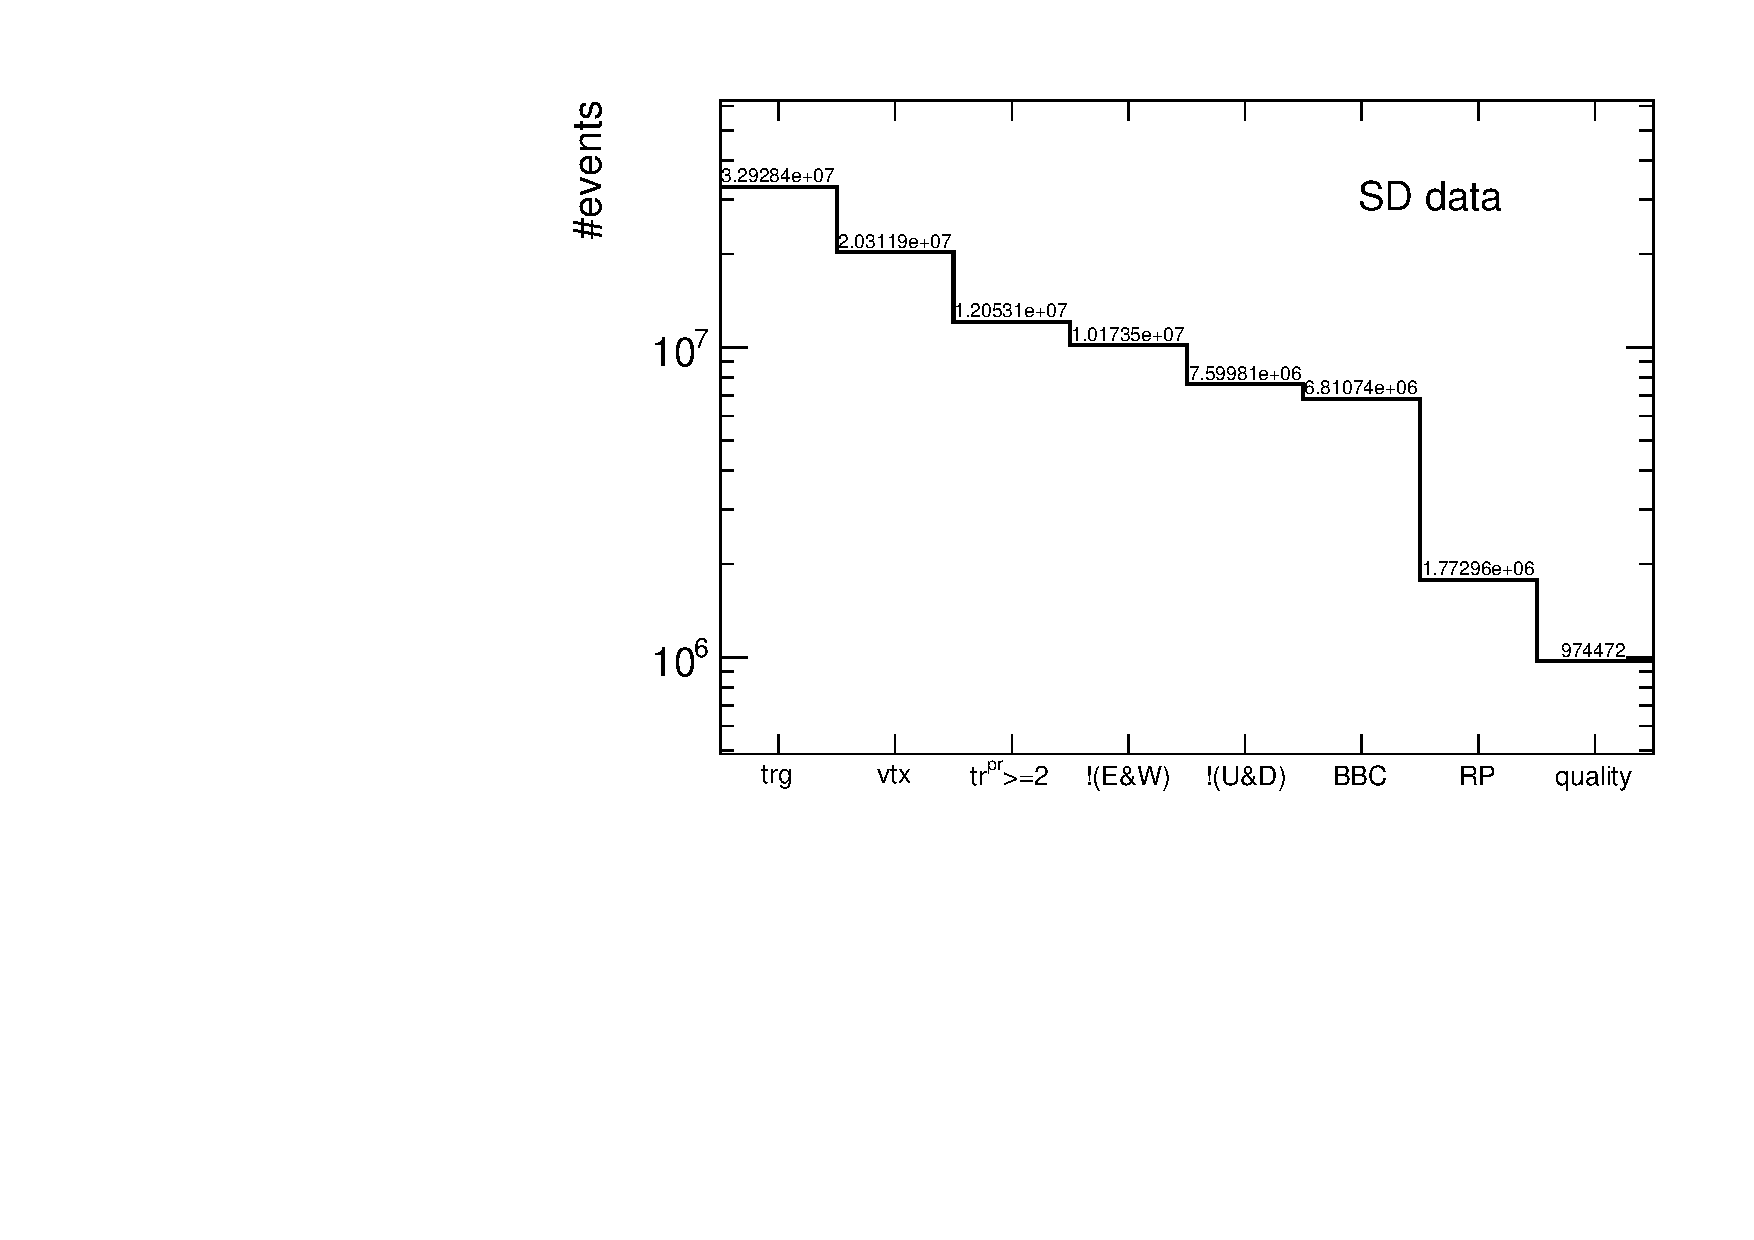
\includegraphics[width=1.04\linewidth, page=1]{graphics/cutFlow/SDT.pdf}}}
		\end{subfigure}
	}
	\quad
	\parbox{0.484\textwidth}{
		\centering
		\begin{subfigure}[b]{\linewidth}{
				{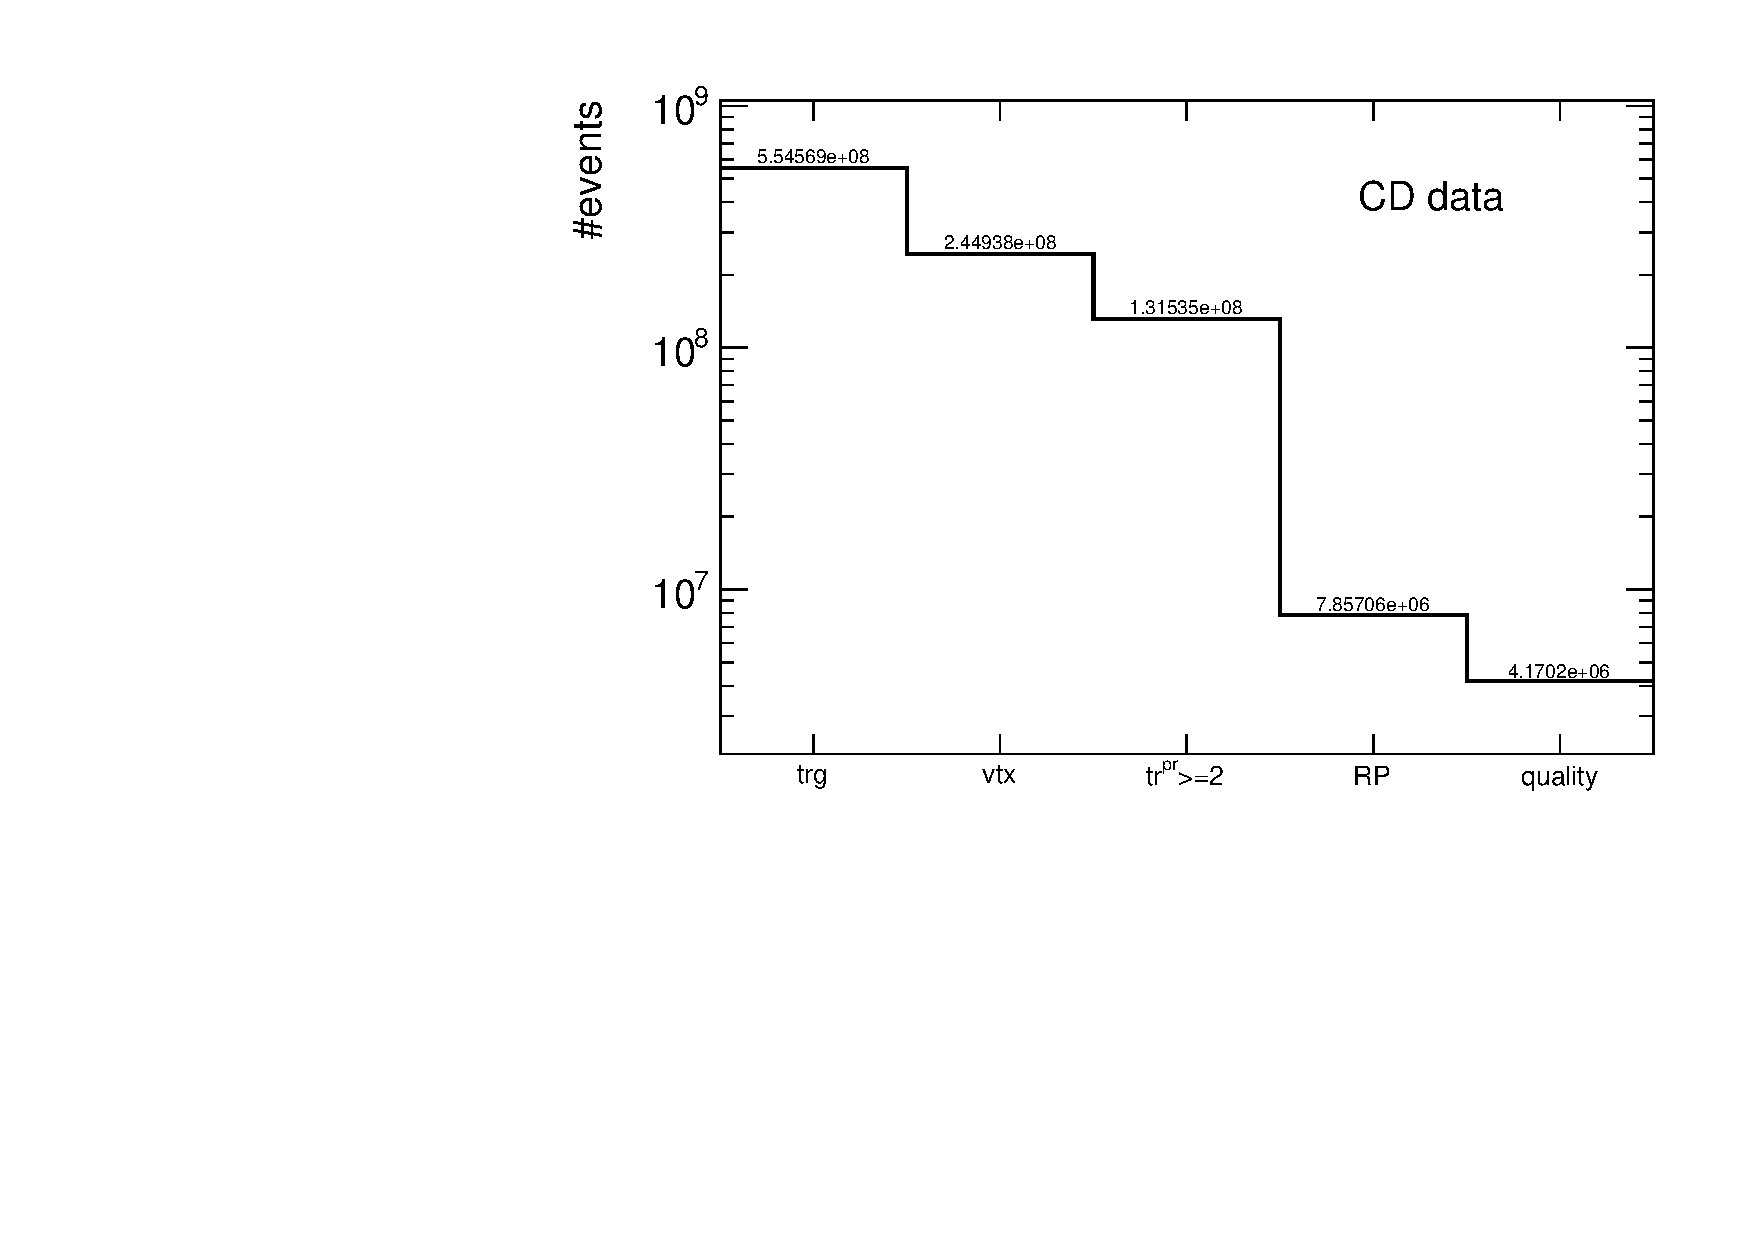
\includegraphics[width=1.04\linewidth, page=1]{graphics/cutFlow/CPT2.pdf}}}
		\end{subfigure}
	}
	\caption[...]{...}
	\label{fig:selectionCutFlow}
\end{figure}
